% LaTeX file for Chapter 06




\chapter{Appendix}


To do:

- include results of ITE estimation with not tuned RF for scenario 1 (fully observed,strong effects) to show the importance that models should be well calibrated (in this case tuned) to yield good results

- inlcude Example of ITE simulation with tram dags with complex shift: $theta + LS(X2) + CS(T, X1)$ to show how tram dags can model interactions. Maybe just refer in the methods for the CS of tram dags, or alternatively in the ITE with tram dags (where i used CI, but to show that CS is also possible to allow for specific interactions)




\section{Negative Log Likelihood}


\subsection{Continuous Outcome}

% Emphasized core components
For a continuous outcome Y the CDF is given by:

\begin{equation}
F_{Y \mid \mathbf{X} = \mathbf{x}}(y) = F_Z(h(s(y) \mid \mathbf{x}))
\end{equation}

where in our case \( F_Z \) is the cumulative distribution function of the standard logistic distribution

\begin{equation}
F_Z(z) = \frac{1}{1 + e^{-z}}, \quad z \in \mathbb{R}
\end{equation}

and \( h \) is the conditional transformation function that maps the scaled outcome \( s(y) \) to the latent scale Z (log-odds).

The outcome $y$ has to be scaled onto the range $[0, 1]$, because the Bernstein polynomial is bounded:

\begin{equation}
s(y) = \frac{y - \min(y)}{\max(y) - \min(y)}
\end{equation}

This scaling also has to be considered when taking the derivative to get the PDF with the change of variables formula:

\begin{equation}
f_{Y \mid \mathbf{X} = \mathbf{x}}(y) = f_Z(h(s(y) \mid \mathbf{x})) \cdot h'(s(y) \mid \mathbf{x}) \cdot s'(y)
\end{equation}

Where $f_Z$ is the PDF of the standard logistic distribution:

\begin{equation}
f_Z(z) = \frac{e^{z}}{(1 + e^{z})^2}, \quad z \in \mathbb{R}
\end{equation}

Finally, the NLL-contributions are then given by the negative log-densities evaluated at the observations.

\begin{equation}
\text{NLL} = - \log (f_{Y \mid \mathbf{X} = \mathbf{x}}(y))
\end{equation}

The full formula is given by

\begin{align}
\text{NLL} = - \log f_{Y \mid \mathbf{X} = \mathbf{x}}(y)
&= -h(s(y) \mid \mathbf{x}) - 2 \log(1 + \exp(-h(s(y) \mid \mathbf{x}))) \nonumber \\
&\quad + \log h'(s(y) \mid \mathbf{x}) - \log(\max(y) - \min(y))
\end{align}




\subsection{Discrete Outcome}


The for a discrete outcome (binary, ordinal, categoric) with categories $y_k$, $k = 1, \ldots, K$, the CDF is given by:

\begin{equation}
F(Y_k \mid \mathbf{X}) = F_Z(h(y_k \mid \mathbf{x}))
\end{equation}

The likelihood contributions are then given by

\begin{equation}
l_i(y_k \mid \mathbf{x}) = f_{Y_k \mid \mathbf{X} = \mathbf{x}}(y_k) =
    \begin{cases}
      F_Z(h(y_k \mid \mathbf{x})) & k=1\\
      F_Z(h(y_k \mid \mathbf{x})) - F_Z(h(y_{k-1} \mid \mathbf{x})) & k=2,\ldots, K-1\\
      1- F_Z(h(y_{k-1} \mid \mathbf{x})) & k = K
    \end{cases}
\end{equation}


from which the NLL-contributions are derived

\begin{equation}
\text{NLL} = - \log (f_{Y_k \mid \mathbf{X} = \mathbf{x}}(y)
\end{equation}


\section{Interpretation of Linear Coefficients} \label{sec:interpretation_linear_coefficients}

The transformation model framework allows for interpretation of the coefficients in the linear shift. Consider the conditional transformation function:

\begin{equation}
F_{X_2 \mid X_1}(x_2) = \operatorname{expit}( h(x_2) + \beta_{12} x_1 ),
\end{equation}

where \( h(x_2) \) is a smooth, monotonic transformation (e.g., a Bernstein polynomial), and \( \beta_{12} \) is a linear coefficient encoding the effect of \( X_1 \) on \( X_2 \).

Taking the logit (inverse expit) yields:

\begin{equation}
\log\left( \frac{F_{X_2 \mid X_1}(x_2)}{1 - F_{X_2 \mid X_1}(x_2)} \right)
= h(x_2) + \beta_{12} x_1.
\end{equation}

This linear additive structure allows the interpretation of \( \beta_{12} \). The odds ratio when increasing \( x_1 \) by one unit is:

\begin{equation}
\text{OR}_{x_1 \to x_1 + 1} = 
\frac{\exp(h(x_2) + \beta_{12}(x_1 + 1))}{\exp(h(x_2) + \beta_{12} x_1)} 
= \exp(\beta_{12}).
\end{equation}

\noindent\textbf{Interpretation:} The quantity \( \exp(\beta_{12}) \) represents the \textbf{multiplicative change in odds} for \( X_2 \le x_2 \) when increasing \( X_1 \) by one unit, holding all else constant.



\section{Encoding of discrete variables} \label{sec:encoding_discrete_variables}

In the TRAM-DAG a variable $X_i$ can act as a predictor variable for a child node, or as an outcome (child node) that depends on some parent nodes. When $X_i$ is acting as an outcome, the distribution of the variable $X_i$ represented by the transformation function $h$ which estimates a cut-point for each variable. So different form of intercept $h_i$ is used compared to a continuous outcome variable.

If a discrete variable $X_i$ with $K$ categories is used as a predictor variable, it should be dummy encoded. This is done by creating $K-1$ binary variables, where each variable indicates whether the observation belongs to this specific category/level or not. The first category/level is used as the reference and is not explicitly included in the model.

Example: for an ordinal variable $X_i$ with three levels (1, 2 3), we create two binary variables:

\begin{itemize}
  \item $X_{i,1}$: 1 if $X_i = 2$, 0 otherwise
  \item $X_{i,2}$: 1 if $X_i = 3$, 0 otherwise
\end{itemize}

Assume a continuous outcome $Y$ that depends on the ordinal variable $X$ with 3 levels, the CDF for $Y$ is given by: 
$F(Y \mid X=1) = F_Z(h_I(y) + x_1\beta_1 + x_2\beta_2)$ 

For $X=1$, the reference level, the CDF simplifies to: 
$F(Y \mid X=1) = F_Z(h_I(y))$

For $X=2$, the CDF becomes: $F(Y \mid X=1) = F_Z(h_I(y) + \beta_1)$

For $X=3$, the CDF becomes: $F(Y \mid X=1) = F_Z(h_I(y) + \beta_2)$

The coefficients $\beta_1$ and $\beta_2$ can be interpreted as the additive shift in the latent scale $h_I(y)$ when moving from the reference level (1) to levels 2 and 3, respectively.


\section{Scaling of continuous variables} \label{sec:scaling_continuous_variables}

Neural networks work best when the input variables are standardized. A linear, monotonic and invertible transformation of a predictor variable changes the interpretation of the coefficient. Scaling a predictor variable $X$ as $X_{\text{std}} = (X - mean(X)) / sd(X)$ will imply that the coefficient $\tilde{\beta}$ is interpreted as the change in log-odds for a one standard deviation increase in the predictor variable or equivalently, for a one unit increase in the standardized predictor. This is different from the interpretation of the coefficient $\beta$ in the original scale, which represents the change in log-odds for a one unit increase in the predictor variable.




In contrast, the standardization of the outcome variable has no effect on the interpretation (because the scale invariance of the log-odds). Consider, we standardize the outcome \( Y \) as follows:

\[
Y_{\text{std}} = \frac{Y - \mu_Y}{\sigma_Y}
\]

This transformation is linear, monotonic, and invertible:

\[
Y = Y_{\text{std}} \cdot \sigma_Y + \mu_Y
\]

Therefore, for any threshold \( y \), we have the equivalence:

\[
P(Y < y \mid X) = P\left(Y_{\text{std}} < \frac{y - \mu_Y}{\sigma_Y} \mid X\right)
\]

This means that the probability is the identical when evaluating the same quantile in the standardized outcome as in the raw outcome. Furthermore, the interpretation of coefficients in a continuous outcome logistic regression remains unchanged. In particular, the log-odds ratio:

\[
\log \left( \frac{P(Y < y \mid X + 1)}{1 - P(Y < y \mid X + 1)} \right) -
\log \left( \frac{P(Y < y \mid X)}{1 - P(Y < y \mid X)} \right)
\]

is equal to:

\[
\log \left( \frac{P\left(Y_{\text{std}} < \frac{y - \mu_Y}{\sigma_Y} \mid X + 1\right)}{1 - P\left(Y_{\text{std}} < \frac{y - \mu_Y}{\sigma_Y} \mid X + 1\right)} \right) -
\log \left( \frac{P\left(Y_{\text{std}} < \frac{y - \mu_Y}{\sigma_Y} \mid X\right)}{1 - P\left(Y_{\text{std}} < \frac{y - \mu_Y}{\sigma_Y} \mid X\right)} \right)
\]

as long as the same quantile (i.e. probability threshold) is used. Thus, the coefficient \( \beta \) reflects the same change in log-odds for a one-unit increase in the (standardized) predictor, regardless if the outcome is standardized or not. This property is also crucial for the evaluation of the bernstein polynomial, since the outcome has to be scaled on a range between 0 and 1.


The general formula of the transformation model is

\[
P(Y < y \mid X = x) = F_z\left(h(Y) + \beta \cdot X\right)
\]

but the model is fitted with standardized outcome and predictors

\[
P(Y_{\text{std}} < y_{\text{std}} \mid X_{\text{std}} = x_{\text{std}}) = F_z\left(\tilde{h}(Y_{\text{std}}) + \tilde{\beta} \cdot X_{\text{std}}\right)
\]

where $\tilde{h}$ and $\tilde{\beta}$ represent the estimated transformation function and coefficients after standardizing the outcome and predictors.

For example, if we want to know the probability \( P(Y < 20 \mid X = 3) \) with standardized variables, the model is specified as

\[
P\left(\frac{Y - \mu_Y}{\sigma_Y} < \frac{20 - \mu_Y}{\sigma_Y} \,\middle|\, X_{\text{std}} = \frac{3 - \mu_X}{\sigma_X} \right)
= F_z\left(\tilde{h}\left(\frac{20 - \mu_Y}{\sigma_Y}\right) + \tilde{\beta} \cdot \frac{3 - \mu_X}{\sigma_X} \right)
\]


\section{Bernstein Polynomial for Continuous Outcomes}

In deep TRAMs the intercept for continuous variables is a smooth monotonically increasing function that is represented by a Bernstein polynomial of order \( K \) (here the complex intercept case where the Intercept already depends on the predictors $x$, however, the same principle that follows also applies for the simple intercept case):

\begin{equation}
h_I(y \mid \mathbf{x}) = \sum_{k=0}^{K} b_k(\mathbf{x}) \cdot B_k(s(y))
\label{eq:bernstein_intercept}
\end{equation}

where \( B_k(s(y)) \) is the Bernstein basis polynomial of order \( K \) evaluated at the scaled outcome \( s(y) \):


To guarantee that the transformation \( h_I(y \mid \mathbf{x}) \) is monotonically increasing in \( y \), the coefficients \( b_k(\mathbf{x}) \) must form a non-decreasing sequence. This is ensured via a *cumulative softmax* parameterization. Instead of learning \( b_k(\mathbf{x}) \) directly as the outputs of the intercept neural network, we first define unbounded parameters \( \theta_k(\mathbf{x}) \in \mathbb{R} \) and then compute the Bernstein parameters using the cumulative softmax transformation:

\begin{equation}
\tilde{b}_k(\mathbf{x}) = \sum_{j=0}^{k} \frac{\exp(\theta_j(\mathbf{x}))}{\sum_{\ell=0}^{K} \exp(\theta_\ell(\mathbf{x}))}, \quad \text{for } k = 0, \ldots, K.
\end{equation}

This transformation produces a vector \( \tilde{b}_k(\mathbf{x}) \) that is monotonically increasing in \( k \), with values bounded in \( [0, 1] \). It ensures that:

- \( \tilde{b}_0(\mathbf{x}) \leq \tilde{b}_1(\mathbf{x}) \leq \ldots \leq \tilde{b}_K(\mathbf{x}) \),
- The sum of increments is 1,
- The transformation is smooth and differentiable.


The combination of Bernstein polynomials with cumulative softmax-transformed parameters allows flexible, smooth, and strictly monotonic transformations of continuous outcomes, which are essential properties for distribution estimation and generative sampling within the deep TRAM architecture.

\subsection{Scaling and Extrapolation of the Bernstein Polynomial}



% :

% \begin{equation}
% s(y) = \frac{y - \min(y)}{\max(y) - \min(y)}
% \end{equation}
Because the Bernstein polynomial is only defined on the range \( [0, 1] \) the outcome y has to be scaled onto the same range. Furthermore, for the sole purpose of estimating the parameters of the Bernstein polynomial it would be sufficient to finish here. However, one has to be able to also evaluate $h(y \mid \mathbf{x})$ for arbitrary values of y, in particular also the ones that are outside of $(\min(y_{train}), \max(y_{train}))$). This is also crucial for sampling. Therefore we extend the Bernstein polynomial by linearly extrapolating the tails of the polynomial. We do this by constructing inside the 5\% and 95\% quantiles of $y$ by the smooth Bernstein polynomial \ref{eq:bernstein_intercept} and linearly extrapolating the outside this range using the slope of the polynomial at the boundaries. This results in a piecewise-defined function that is differentiable, monotonic, and defined for all real values of \( y \), which is essential for evaluating the model at arbitrary outcomes or for generative sampling.

Tho formalize this, let \( q_{0.05} \) and \( q_{0.95} \) denote the 5\% and 95\% empirical quantiles of the outcome \( y \), computed on the training data. The scaled outcome is defined as

\begin{equation}
s(y) = \frac{y - q_{0.05}}{q_{0.95} - q_{0.05}}.
\end{equation}

This scaling maps the interval \( [q_{0.05}, q_{0.95}] \) to the unit interval \( [0, 1] \), which is the domain of the Bernstein basis polynomials. Let \( h_I(s(y) \mid \mathbf{x}) \) be the original transformation as defined in Equation~\eqref{eq:bernstein_intercept}. The extrapolated transformation \( h^*(y \mid \mathbf{x}) \) is then defined as

\begin{equation}
h^*(y \mid \mathbf{x}) =
\begin{cases}
h_I(0 \mid \mathbf{x}) + h_I'(0 \mid \mathbf{x}) \cdot (s(y) - 0), & \text{if } s(y) < 0 \\
h_I(s(y) \mid \mathbf{x}), & \text{if } 0 \leq s(y) \leq 1 \\
h_I(1 \mid \mathbf{x}) + h_I'(1 \mid \mathbf{x}) \cdot (s(y) - 1), & \text{if } s(y) > 1
\end{cases}
\label{eq:extended_bernstein}
\end{equation}

The function is thus extrapolated beyond the central range using the tangent line at the boundaries. The derivatives \( h_I'(0 \mid \mathbf{x}) \) and \( h_I'(1 \mid \mathbf{x}) \) are computed analytically from the Bernstein basis and the learned coefficients \( b_k(\mathbf{x}) \), and ensure continuous differentiability across the domain (see next subsection).


This construction ensures several desirable mathematical properties. First, the transformation \( \tilde{h}(y \mid \mathbf{x}) \) is globally defined on \( \mathbb{R} \), avoiding undefined regions or discontinuities. Second, it preserves monotonicity due to the use of the cumulative softmax parameterization of the coefficients \( b_k(\mathbf{x}) \), which guarantees that the Bernstein polynomial is strictly increasing. Finally, the piecewise-linear extrapolation ensures the function is continuously differentiable and smooth at the junctions \( s(y) = 0 \) and \( s(y) = 1 \).




\subsection{Analytical Derivative of the Bernstein Polynomial Transformation}

To efficiently compute the gradient of the transformation \( h_I(y \mid \mathbf{x}) \) with respect to its inputs, we can exploit the analytical structure of the Bernstein basis polynomials. Recall the general form of the transformation:

\begin{equation}
h_I(y \mid \mathbf{x}) = \sum_{k=0}^{K} b_k(\mathbf{x}) \cdot B_k(s(y)),
\end{equation}

where \( B_k(s) \) are the Bernstein basis polynomials of order \( K \), and \( b_k(\mathbf{x}) \) are predictor-dependent coefficients. For fixed \( \mathbf{x} \), the derivative with respect to \( y \) is needed, for example, to evaluate the density function when \( h_I \) is used in a generative model.

Let us denote \( s = s(y) \). Using the chain rule, we compute:

\begin{equation}
\frac{d}{dy} h_I(y \mid \mathbf{x}) = \sum_{k=0}^{K} b_k(\mathbf{x}) \cdot \frac{d}{dy} B_k(s) = \sum_{k=0}^{K} b_k(\mathbf{x}) \cdot \frac{dB_k(s)}{ds} \cdot \frac{ds}{dy}.
\end{equation}

The derivative of the scaled outcome \( s(y) = \frac{y - q_{0.05}}{q_{0.95} - q_{0.05}} \) is simply

\begin{equation}
\frac{ds}{dy} = \frac{1}{q_{0.95} - q_{0.05}}.
\end{equation}

The derivative of the Bernstein basis polynomial \( B_{k,K}(s) \) is known and given by:

\begin{equation}
\frac{d}{ds} B_{k,K}(s) = K \left[ B_{k-1,K-1}(s) - B_{k,K-1}(s) \right].
\end{equation}

Therefore, the full derivative is:

\begin{equation}
\frac{d}{dy} h_I(y \mid \mathbf{x}) = \frac{K}{q_{0.95} - q_{0.05}} \sum_{k=0}^{K} b_k(\mathbf{x}) \left[ B_{k-1,K-1}(s) - B_{k,K-1}(s) \right].
\end{equation}

This expression can be evaluated efficiently and is used both in the likelihood computation (e.g., via change-of-variables) and for constructing tail extrapolations with matching slopes.


\section{Default Random Forest for ITE Estimation} \label{sec:default_rf_ite}

In Section \ref{sec:ite_models} we pointed out the importance of calibration of models when estimating individual treatment effects. In this section we show the results of the default random forest model without tuning for scenario (1), illustrated in Figure \ref{fig:fully_observed_dag_rf_appendix} where all variables are observed and there are strong treatment and interaction effects. The results are shown in Figure \ref{fig:fully_observed_glm_rf}. In the scatterplot of true vs. predicted probabilities for $\text{P}(Y_i = 1 \mid  \mathbf{X_i} = \mathbf{x_i}, T_i = t_i)$ in the train set, it is visible that the model does not predict the probabilities accurately, hence is not well calibrated. This poor calibration also translates to the estimated ITEs. In comparison, the results of the tuned random forest in Figure \ref{fig:fully_tuned_rf_tlearner} show that the model is better calibrated and the estimated ITEs are close to the true ITEs. This illustrates the importance of tuning models for ITE estimation, as poor calibration can lead to biased estimates of individualized treatment effects.


\begin{figure}[htbp]
\centering
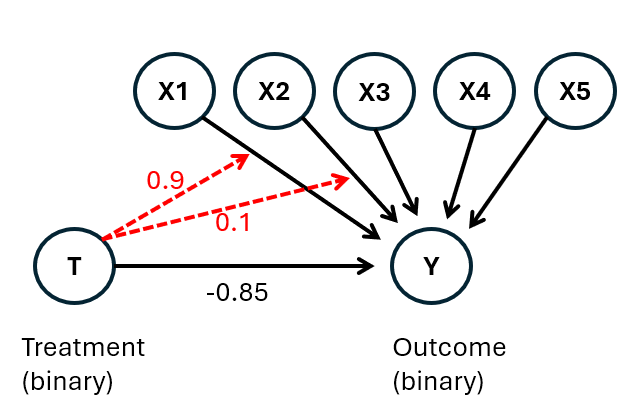
\includegraphics[width=0.35\textwidth]{img/results_ITE_simulation/simulation_observed.png}
\caption{DAG for scenario (1), where all variables are observed and there are strong treatment and interaction effects. The numbers indicate the coefficients on the log-odds-scale. Red: interaction effects between treatment ($T$) and covariates ($X_1$ and $X_2$) on the outcome ($Y$).}
\label{fig:fully_observed_dag_rf_appendix}
\end{figure}


\begin{figure}[htbp]
\centering
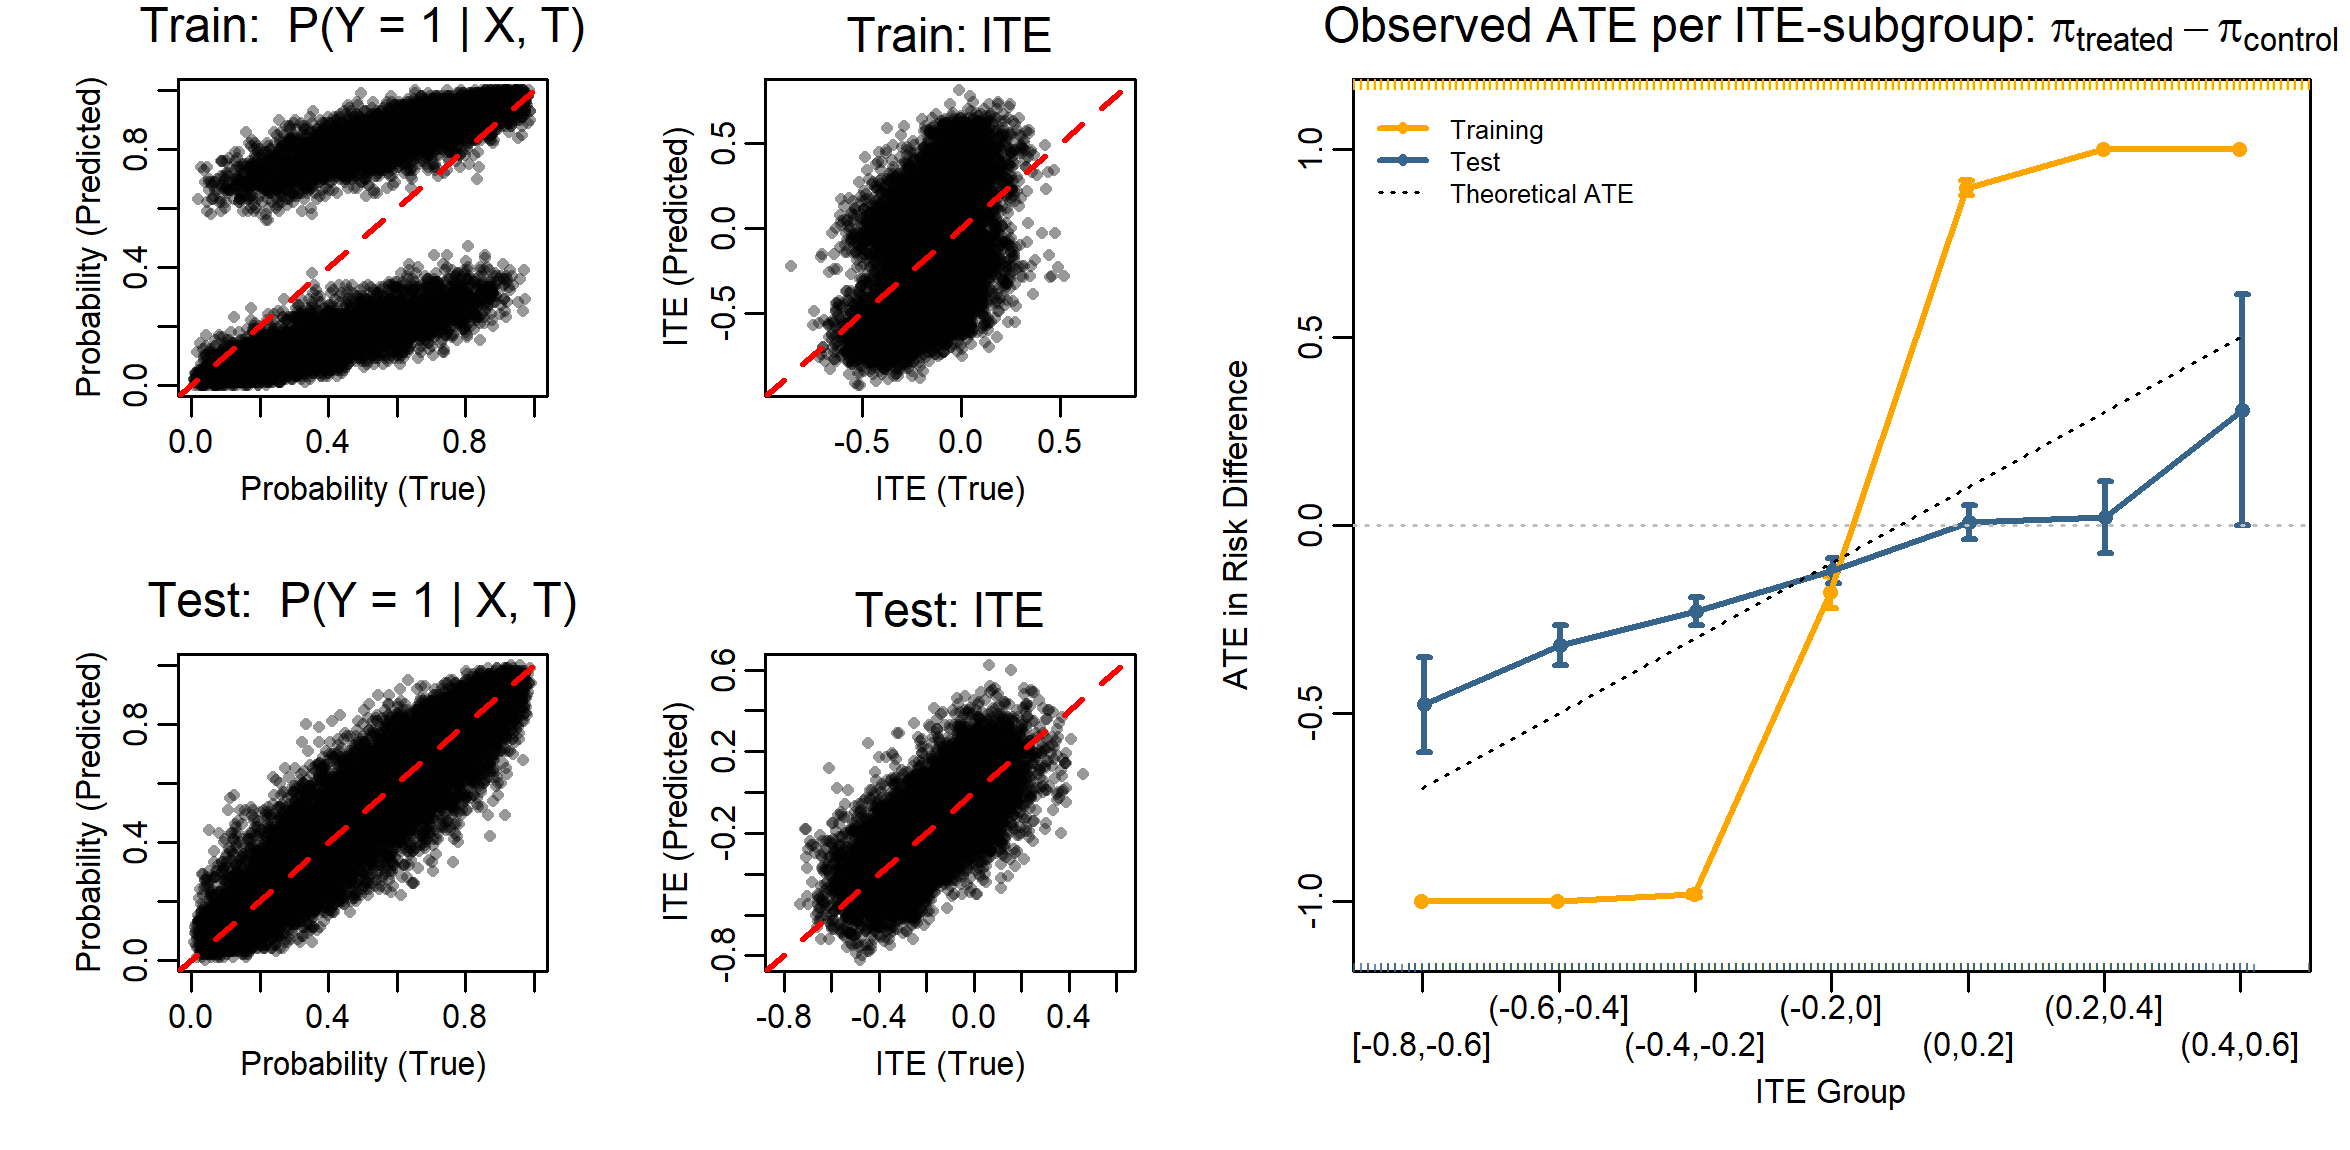
\includegraphics[width=0.9\textwidth]{img/results_ITE_simulation/fully_observed_rf_tlearner.png}
\caption{Results with the default random forest in scenario (1) when the DAG is fully observed and there are strong treatment and interaction effects. Left: true vs. predicted probabilities for $\text{P}(Y=1 \mid X, T)$; Middle: true vs. predicted ITEs; Right: observed ATE in terms of risk difference per estimated ITE subgroup.}
\label{fig:fully_observed_glm_rf}
\end{figure}




\section{Calibration differences for complex model: Experiment 3} \label{sec:calibration_tuned_rf}

Figure \ref{fig:calibration_tuned_rf} shows the calibration plots in terms of the predicted risks against the the observed proportions of the event for the T-learner tuned random forest for scenario (3) with weak direct and interaction treatment effects. This is in contrast to the prediction plots presented in Section \ref{sec:results_experiment3} where we presented the true probabilities of the event $\text{P}(Y=1 \mid X, T)$ against the predicted probabilities. It becomes apparent, that tuning the random forest model out-of-bag leads to a poor calibration on the training set, but due to better generalization it leads to a better calibration on the test set.

\begin{figure}[htbp]
\centering
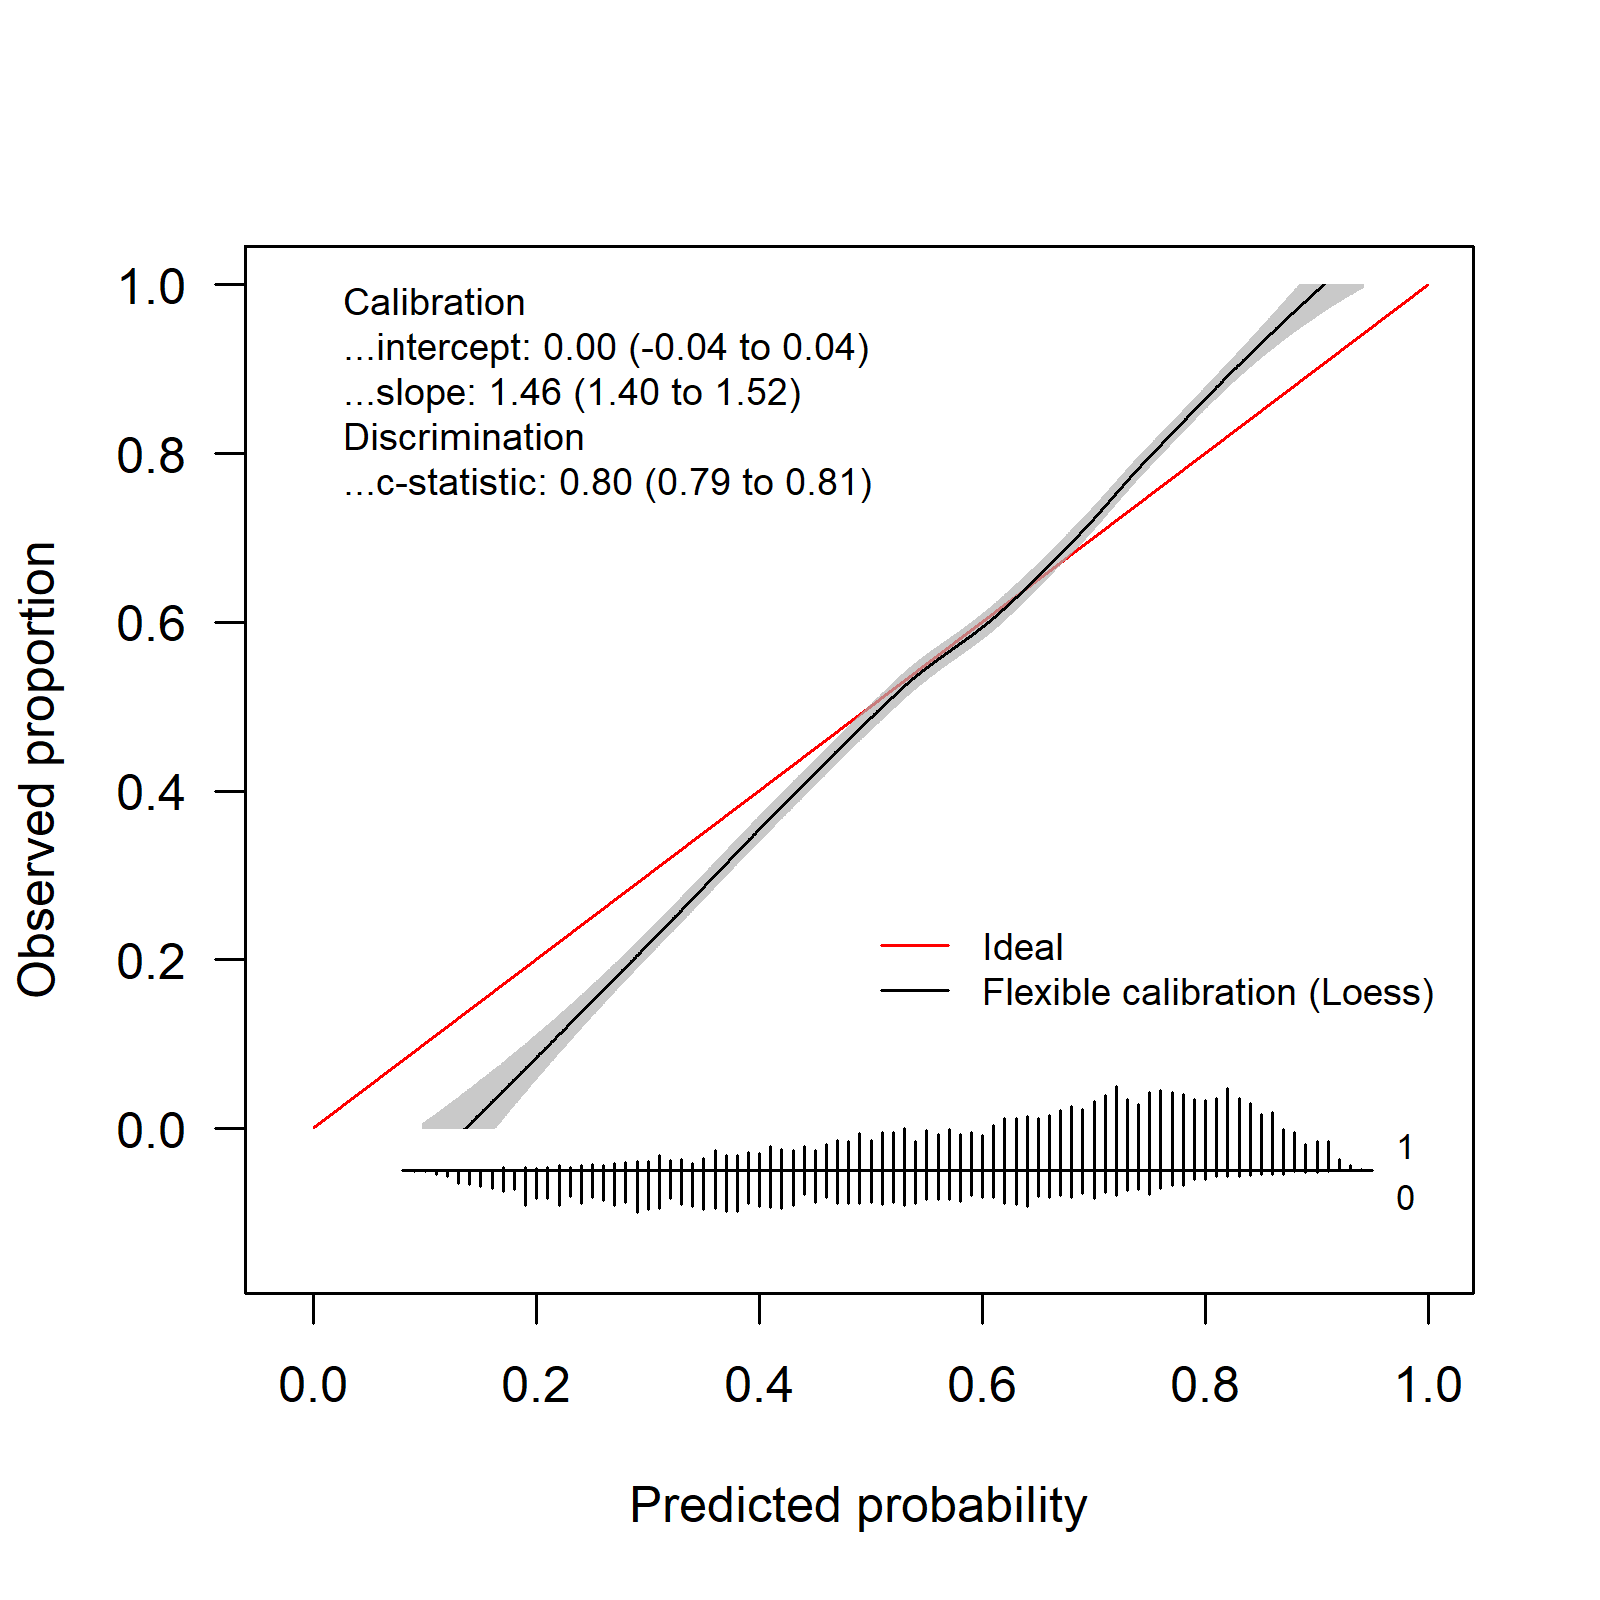
\includegraphics[width=0.45\textwidth]{img/results_ITE_simulation/small_interaction_tuned_rf_tlearnertrain_calibration_plot.png}
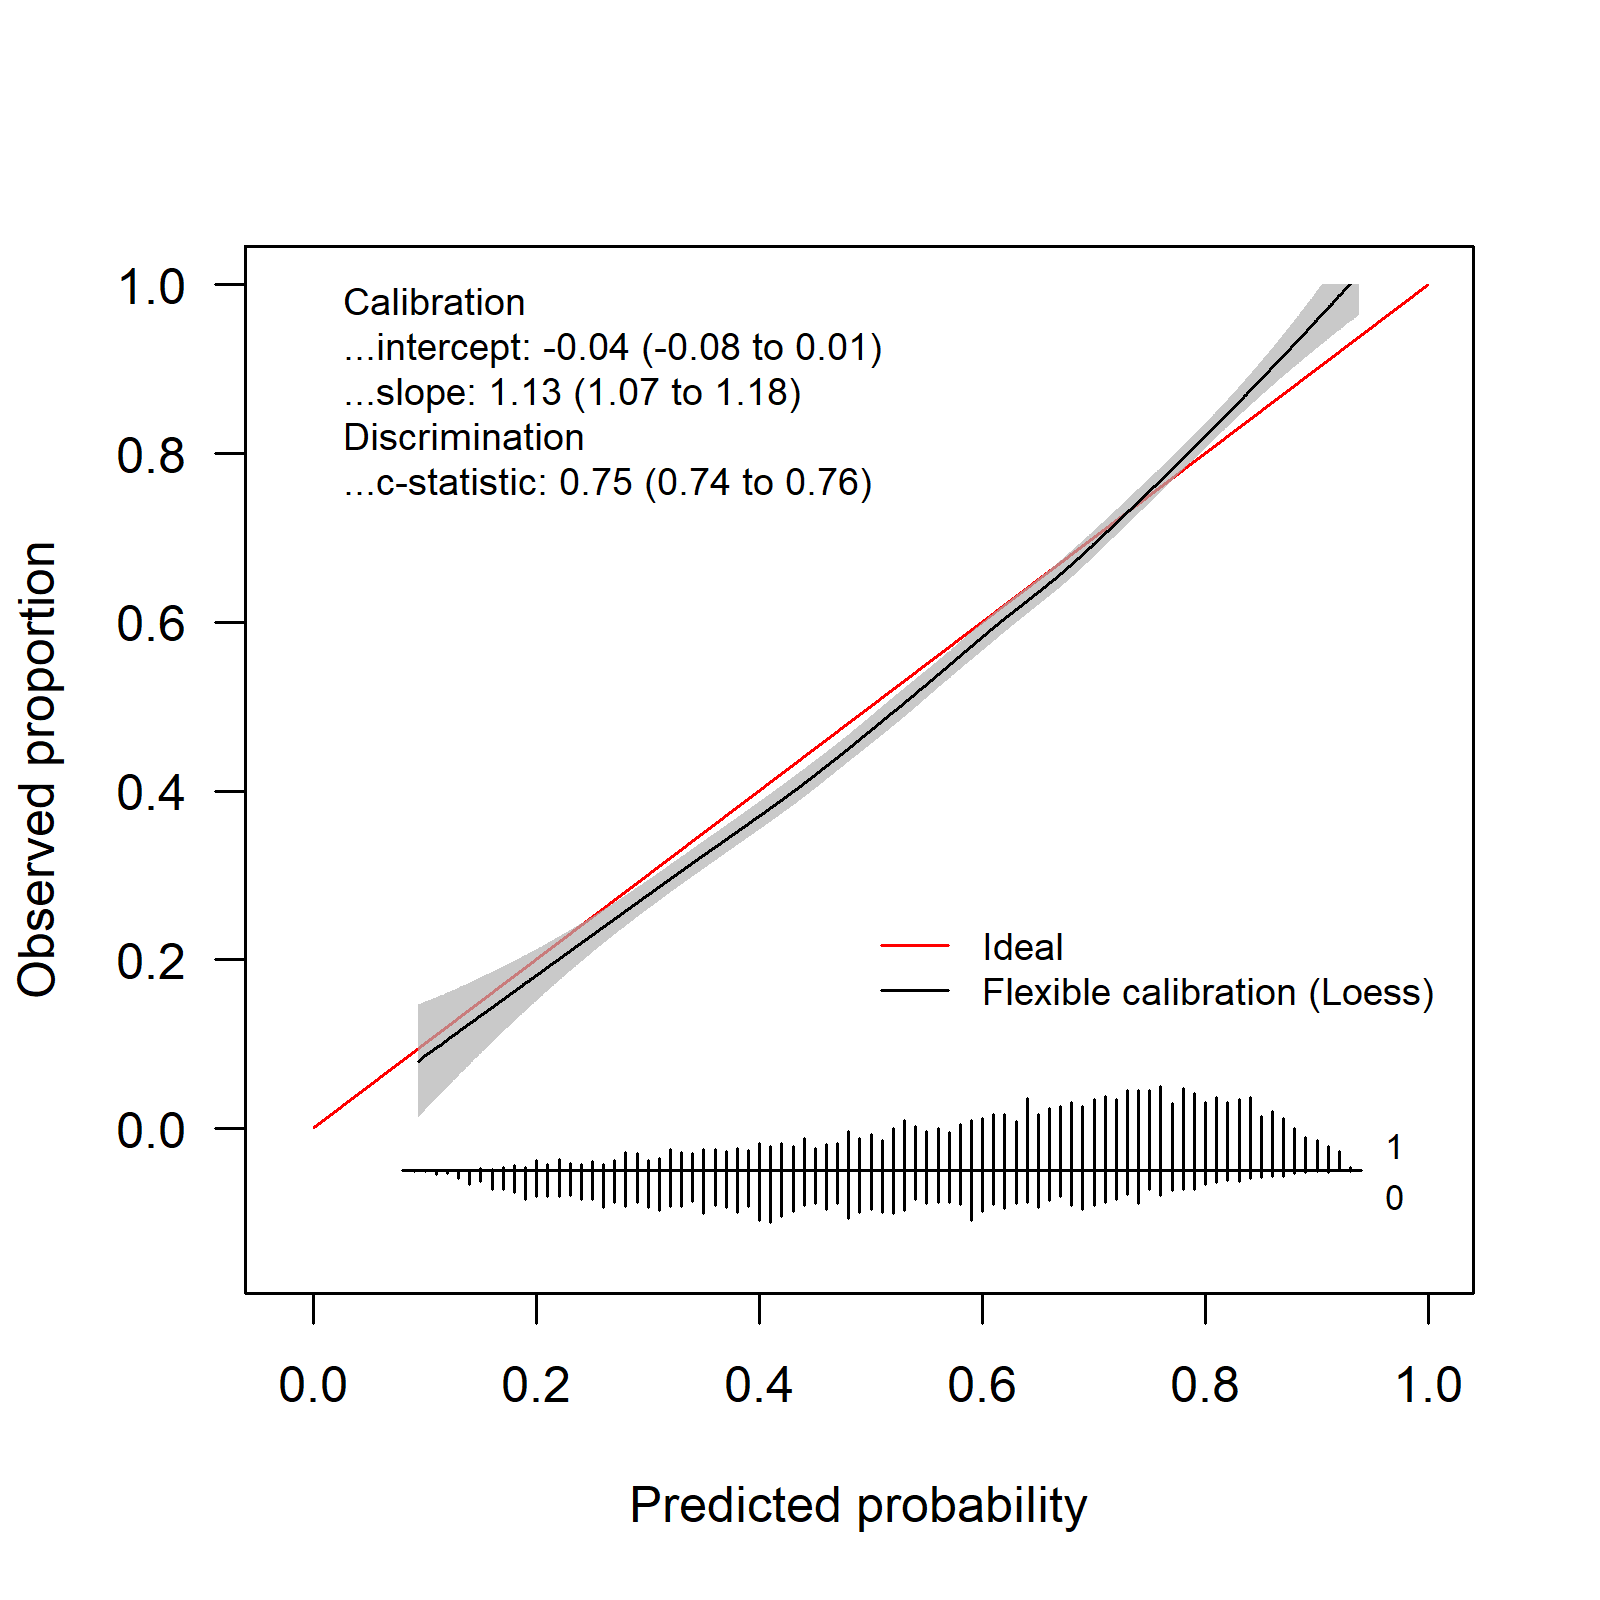
\includegraphics[width=0.45\textwidth]{img/results_ITE_simulation/small_interaction_tuned_rf_tlearnertest_calibration_plot.png}
\caption{Calibration plot for the T-learner tuned random forest for scenario (3) with weak direct and interaction treatmetn effects. It shows the predicted risks against the the observed proportions of the event. Left: training dataset; Right: test dataset.}
\label{fig:calibration_tuned_rf}
\end{figure}


